\documentclass[11pt]{article}
\usepackage[includeheadfoot, top=1.0in, bottom=1.0in, hmargin=1.0in]{geometry}
\usepackage[utf8]{inputenc}
\usepackage{fancyhdr}
\usepackage{url}
\pagestyle{fancy}
\usepackage{setspace}
\usepackage{tabularx}
\usepackage{graphicx}
\usepackage{caption}
\usepackage{subcaption}
\usepackage{hyperref}
\usepackage{multicol}
\usepackage{amsmath}
\usepackage{enumitem}

\usepackage{hyperref}
\hypersetup{
    colorlinks=true,
    linkcolor=blue,
    filecolor=magenta,      
    urlcolor=blue,
}


\lhead{Astronomy Lab II}
\rhead{Fall 2024}
\lfoot{Porter}
\rfoot{Wed 6-9pm}
\cfoot{\thepage}

\begin{document}

\begin{center}
\huge{Makeup Lab: Exoplanets}\\ \medskip \Large{October 23, 2024}
\end{center}

%%%%%%%%%%%%%%%%%%%%%%% INTRO %%%%%%%%%%%%%%%%%%%%%%%
\section{Introduction}
%Maryum

Since the discovery of the first exoplanet in 1992, the field of exoplanets has been revolutionized thanks to NASA's space-based mission, \textit{Kepler}. Launched in 2009, \textit{Kepler} provided a wealth of data on a diversity of systems such as TRAPPIST-1 which hosts 7 planets within the orbit of Mercury, or KOI-5Ab, an exoplanet that orbits a 3-star system. Exoplanets can be discovered through a number of methods, but the two most common methods are the \textit{radial velocity} and the \textit{transit} methods. Later on, we will discuss the biases of each method. While all the initial discoveries were made through the radial velocity methods, \textit{Kepler} quickly provided thousands of additional planet discoveries; now there are 5000+ discovered exoplanets and 7000+ exoplanet candidates. 

\medskip \noindent
With thousands of discovered exoplanets, we can learn a lot about the demographics of exoplanets and their host-stars. For instance, \textit{Kepler} showed us that the majority of stars tend to host close-in planets the size of super-Earths or sub-Neptunes. This is unlike our own and therefore questions the uniqueness of our solar system. In addition, giant planets are more likely to be found around stars with more heavy elements, and small rocky planets are more common than giant planets.  Although \textit{Kepler} was de-commissioned in 2018, the new NASA mission, TESS (Transiting Exoplanet Survey Satellite), is picking up where \textit{Kepler} left off. Launched in 2018, TESS has already found almost 300 planets with 6000+ candidates!


%%%%%%%%%%%%%%%%%%%%%%% TRANSITS %%%%%%%%%%%%%%%%%%%%%%%
\section{Transits: Cosmic Photobombs}
%Ben

In $\sim$25 years of searching, astronomers have tried many techniques to find planets around other stars. However, one of these techniques, the \textbf{transit method}, is the current reigning champion out of them all, if you go by pure number of discoveries alone at least.

\medskip \noindent
So, what exactly is the transit method? Somewhat flippantly, it’s when a planet photobombs a picture we’re taking of a star.

\medskip \noindent
When stars are left alone, they should shine with a steady, constant brightness that we agree on each time we measure them. However, it turns out that most stars have planets which circle around them in clean, repeating patterns. If the orientation of those orbits line up just right, those planets will fall between us and the star once each lap around. From our point of view, they will block a little bit of light from their parent star at the same point in each of their ``years". Our brightness measurements will have appeared to drop when the planet is between us and the star, but then will go back up again once the planet continues on its way. On a graph of time vs. brightness (astronomers refer to these graphs as \textit{light curves}), a transiting planet will look like Figure \ref{fig:transit}. Also check out the animation at the bottom of this page to see how this looks as the planet orbits: \url{https://exoplanets.nasa.gov/faq/31/whats-a-transit/}

\begin{figure}[h!]
    \centering
    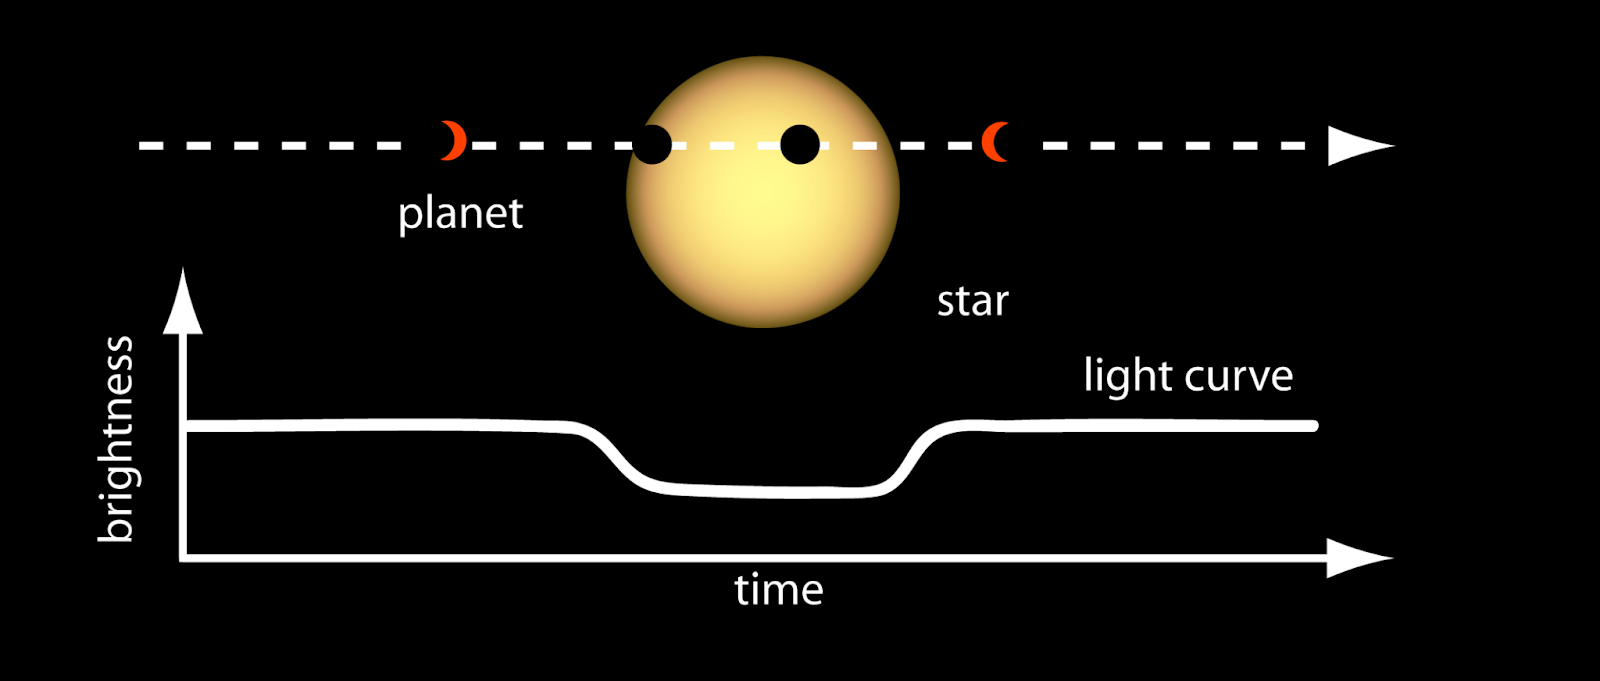
\includegraphics[width=0.9\textwidth]{Images/transit_cartoon.png}
    \caption{Illustration of an exoplanet transit. Credit: NASA}
    \label{fig:transit}
\end{figure}

\medskip \noindent
These graphs are the \textit{only} information we get about a transiting planet. But, as simple as they are, we can learn a lot about a planet from them!  \textbf{Answer the following questions in your lab write-up:}

\begin{enumerate}
    \item What happens to the depth of the ``dip" as the size of the planet gets larger (assume you are looking at the same star)? What would happen to the depth of the ``dip" if instead the size of the planet remained the same, but the star got larger?  Why?
    
    \item Your friend says, ``You can use the transit method to measure the size of a planet without knowing the size of the star." Is your friend right or wrong? Why? What do you think you \textit{can} measure about sizes with the light curve?
    % Dip gets larger too, and no actually, only the ratio of it to the star's radius
    
    \item What happens if a star has planets but their orbits are “tilted” away from us? Would we detect these planets via their transits?
    % Nope, geometric bias
    
    \item You want to measure the \textit{period} of a planet (the time it takes for a planet to complete one lap around its star). Using the transit method, what data would you need in order to do this?
    % Time between dips
    
    % 5
\end{enumerate}

\subsection{Your Very Own Transit}
\noindent
We’re now going to try to get a better sense of how this method works in practice. This portion of the lab directs at least one member of your group to stand on a stool -- if that is infeasible or would cause discomfort, please let me know.  

\begin{enumerate}
\setcounter{enumi}{4}
    \item Follow all of the following steps and \textbf{record your results in your lab write-up.}
\end{enumerate}

\begin{enumerate}[label=Step \arabic*:]
    \item Have at least one member download an app which can use your phone’s camera to measure brightness (Android users, I recommend Light Meter Free; Apple users, I recommend LUX Light Meter Free). Plenty of these apps exist for photographers, but make sure you get one which uses your phone’s camera, not its light meter.
    
    \item Get a paper towel roll, or roll up/tape a piece of paper into a similar shape, then move to someplace in the room where when looking through the tube you can isolate a single one of the weird orb overhead lights (ideally one of the lower ones). This will be your target ``star"!
    
    \item Pick one of the styrofoam balls, which will be your ``planet" to detect.
    
    \item Have one member hold the tube over their camera’s lens so that just the ``star" is in view. Then, take 8 measurements of the brightness of the star. We do this since no measurement is perfect, and these apps can be finicky- real issues astronomers face with telescopes too! Write down each of your measurements in your lab notebook.
    
    \item Now, with another member standing on a stool within reach of the star, have them hold the “planet” in front of light. Take another 8 measurements, trying to change as little about the scene as possible between readings, recording these as well.
    
    \item Before stepping down, use a string and a yard stick or a flexible tape measure to record the circumference of your ``star" (the distance around the widest part).
\end{enumerate}

\noindent
Congratulations, you’ve just taken a transit measurement! Now comes the scientific analysis, let’s see what we can learn about this “planet”. First, some data science. 
\begin{enumerate}[label=Step \arabic*:,resume]
    \item Start by throwing out the highest and lowest measurements in both of your data sets, then take the average of the remaining 6 in each.
\end{enumerate}

\noindent
These are steps taken when looking at real light curves too. We always start by discarding outliers, or points that are so far from all the others we suspect something strange happened during that measurement. We take the average because we’re never completely confident in a single measurement, but we can decrease our uncertainty by considering more measurements. If your “without planet” average is lower than your “with planet” average, let me know and I will give you the backup data- something has gone wrong with your data collection (likely just the sensitivity of the app)! 

\medskip \noindent
Now, some math! Transit analysis pivots around measuring how much light was blocked by your star. We can “normalize” the amount of light we measured by calling the out-of-transit measurements 100\%. To measure the influence of the planet:
\begin{enumerate}[label=Step \arabic*:,resume]
    \item Divide your ``with planet" average by your ``without planet" average.  Let's call this number d.  The \textit{depth} of the transit is 1 - d.
\end{enumerate}

\noindent
You might have guessed that the depth of the transit depends on the area we see of the star and the area we see of the planet. With some rearrangement, we can use our measurement of the star’s size and the transit’s depth to get a measurement of the planet’s size! First, we need to calculate the area of your star.

\begin{enumerate}[label=Step \arabic*:,resume]
    \item Using the circumference, C, that you measured for your star, calculate the radius, R (\textit{hint: }$R = \frac{C}{2\pi}$).
    \item The area of a circle (which is how a star appears to us on the sky) is $A = \pi R^2$.  Solve for the area, A, of your star.
\end{enumerate}

\medskip \noindent
Now we can combine that area and the measured depth into an estimate of the planet's size. The planet can be thought of as ``negative area" when it's in front of the star, something which blocks a small patch we would have otherwise seen. 
\begin{enumerate}[label=Step \arabic*:,resume]
    \item Multiply your transit depth by the area of your star -- this is the area your planet blocks, while it transits, or in other words, the area of your planet!

    $$\text{Planet Area} = (\text{1 - d}) \times \text{A}$$
    
    \item Using this area, solve for the radius of your planet (\textit{hint: }rearrange the equation for A from step 10) This is your measured planet radius! Now, measure the circumference of your planet and calculate its radius the same way you did with your star in step 9.

\end{enumerate}


\medskip \noindent
Some final things to consider:
\begin{enumerate}
\setcounter{enumi}{5}
    \item Is the radius you derived from brightness measurements similar to the one you actually measured when holding the planet? If not, do you have any ideas for why that might be?
    
    %item In an actual transit, what do you think would happen if you accidentally had 2 stars in view, but the planet still orbited just one? Would your without-planet measurements be higher or lower? What about your with-planet measurements? Transit depth (and thereby planet radius)? This is a real problem astronomers worry about, called {\it blending.}
    % The out of transit flux increases, but the dip is the same absolute size, so the ratio is smaller. We'd underestimate the size of the planet 
\end{enumerate}


%%%%%%%%%%%%%%%%%%%%%%% RV %%%%%%%%%%%%%%%%%%%%%%%
\section{Wadial Wobbles: The Radial Velocity Method}
\subsection{Predictions} \label{sec:RV_predictions}

In our Spectroscopy lab, you learned how we can use the spectral lines of different elements to figure out how fast an object is moving towards or away from us.  In short, the faster something is moving away from us, the more \textit{redshifted} its spectral lines will be, and the faster something is moving towards us, the more \textit{blueshifted} its spectral lines will be.  When we study redshift in galaxies, we witness large-scale deviations in spectral lines on the order of 100s or 1000s of Angstroms (velocities of order $10^8$ km/s).  However, redshift and blueshift are not confined to large-scale motions, and we can use these same techniques to detect \textit{radial velocity (RV)} motions in nearby stars caused by the gravitational tugs of their planetary companions.  These small tugs mean that we are looking at velocities on the order of a few tens of km/s and so the deviations in the spectral lines are \textit{minuscule}. Let's think about how the radial velocity method works with planets:

\begin{enumerate}
\setcounter{enumi}{6}
    \item Check out this gif from the Wikipedia page on radial velocity: \url{https://en.wikipedia.org/wiki/Radial_velocity#/media/File:Planet_reflex_200.gif}.  You'll notice that both planet and star orbit around a common \textit{center of mass}, but this point is generally still inside the star itself.  Make a generalized statement that describes how the star moves relative to the planet. Or in other words, where is the star in its orbit at each point of the planet's orbit?
    % The star is fastest when the planet is in quadrature- phase shift from the acceleration vector, a little tricky
        
    \item Let's think about how our orientation relative to the star-planet system affects our ability to take radial velocity measurements.
        \begin{enumerate}
            \item We know that if we view the system edge on ($90^\circ$ inclination), as above, we can see the spectrum shifting because there is motion towards or away from us.  If we slowly decrease the inclination towards a face-on system ($0^\circ$ inclination), would we get more or less shifting of the spectral lines? Why?
            % Less, taking motion outside the plane
            
            \item If we were viewing a system face-on, would we be able to tell there is a planet using radial velocities? Why or why not?
            % Nope, no motion in plane
        \end{enumerate}
        
    \item Finally, let's make some predictions about how a system's properties affect the radial velocity of the star.
    \begin{enumerate}
        \item Holding the \textit{planet} mass constant, if we increase the star's mass, will the star have higher or lower radial velocity? Why?
        % Lower, harder to tug
        \item Holding the \textit{star} mass constant, if we increase the planet's mass, will the star have higher or lower radial velocity? Why?
        % Higher, move ability to tug
        \item Holding the \textit{star and planet} mass constant, if we increase the semimajor axis of planet (distance from the star), will the star have higher or lower radial velocity? Why?
        % Lower, less acceleration
    \end{enumerate}
        
\end{enumerate}

\section{A Plethora of Planets}
Go to the NASA Exoplanet Archive plotting tool (\url{https://exoplanetarchive.ipac.caltech.edu/cgi-bin/IcePlotter/nph-icePlotInit?mode=demo&set=confirmed}).  \textbf{Plot each of the following, and then write a few sentences on what you learn from each plot (what trends do you observe, what do you think they mean, what do large empty spaces on the plot mean/why are observations bias towards the sample that is plotted).}  Use what you now know about the transit and RV methods. \textit{Hint:} Kepler's 3rd law states that the period of a planet's orbit squared is directly proportional to the distance between the star and the planet cubed ($P^2 \propto a^3$). \textbf{Include your plots in your lab write-up.} 
    \begin{enumerate}
    \setcounter{enumi}{9}
        \item Planet Radius (x-axis) vs. Orbital Period (y-axis). %Why is there a the lack of detections for long period, small radius planets?
        % Geometric and size biases both count against transits
        \item Planet Mass (x-axis) vs. Orbital Period (y-axis). %Why is there a the lack of detections for long period, low mass planets? 
        % Both biases count against RVs
    \end{enumerate}


%%%%%%%%%%%%%%%%%%%%%%% CONCLUSIONS %%%%%%%%%%%%%%%%%%%%%%%
\newpage
\section{Wrapping Things Up}

\begin{figure}[h!]
    \centering
    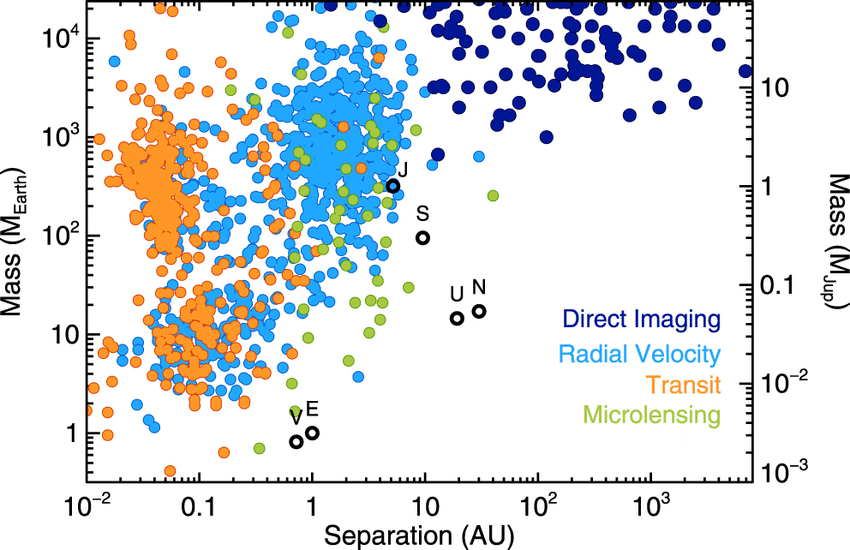
\includegraphics[width=0.8\textwidth]{Images/Exoplanet Demographic Techniques.png}
    \caption{Demographics of exoplanets colored by detection techniques. Credit: Bowler, 2016.}
    \label{fig:techniques}
\end{figure}

Figure \ref{fig:techniques} is a plot of the masses of discovered exoplanets versus their distance from their host stars, colored by the detection method that was used to discover them. Let's think about why certain methods may be biased towards detecting certain types of planets.

\begin{enumerate}
\setcounter{enumi}{11}
    \item Using what you learned in this lab, explain why planets detected with the transit technique are both primarily massive and close to their host stars. 
        
    \item Using this same plot, we see that we can detect planets using the radial velocity method out to larger separations.
    
    \begin{enumerate}
        \item  Why are we able to use the RV method to detect planets further away from their hosts than the transit method? 
            
        \item Why can't we detect small planets far away from their stars using the RV method? 
            
    \end{enumerate}
    
    \item Research the Direct Imaging technique (\url{https://en.wikipedia.org/wiki/Methods_of_detecting_exoplanets#Direct_imaging}) and explain how it works (a few sentences).  Why is Direct Imaging biased towards massive planets far from their hosts?
    
    \item In an exciting turn of events for this lab class, you discovered a planet that is 1 Earth radius and 1 Earth mass in size! You name it ``Planet 1904" after your favorite astronomy lab class. Your friend says ``Wow! Planet 1904 \textbf{must be} habitable!" Is your friend right? Explain why or why not. What else might you need to know about the planetary system to be more confident in it's habitability?  Which quantities (if any) could you determine using the transit or RV method?
     % Depends how far it is from the star, stuff about the star, chemical comp
\end{enumerate}


\end{document}